\documentclass[border=1pt]{standalone}
\usepackage[dvipsnames]{xcolor}
\usepackage{tikz}                       % Graphen und kommutative Diagramme
\usetikzlibrary{patterns}               % Um schraffierte Formen in der tikzpicture-Umgebung zu zeichnen.
\newcommand{\ul}[1]{\underline{\smash{#1}}}

\begin{document}

\centering
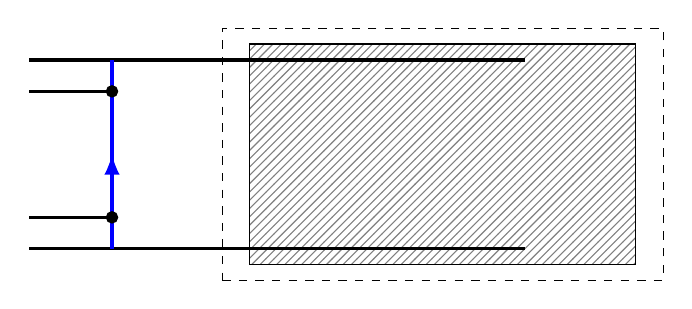
\begin{tikzpicture}[x=.7cm, y=.4cm, line width=.5pt]
    % draw shaded slit box
    \filldraw[pattern=north east lines, pattern color=black!50] (0, 1.5) -- (7, 1.5) -- (7, 8.5) -- (0, 8.5) -- (0, 1.5);
    
    % draw line width=2pt boundary lines
    \draw[dashed] (-.5, 1) -- (7.5, 1) -- (7.5, 9) -- (-.5, 9) -- (-.5, 1);
    
    \draw[line width=1.2pt] (-4, 2) -- (5, 2);
    \draw[line width=1.2pt] (-4, 8) -- (5, 8);
    
    \draw[-latex, color= blue, line width=1.5pt] (-2.5, 2) -- (-2.5,5);
    \draw[color= blue, line width=1.5pt] (-2.5, 4) -- (-2.5,8);
    % draw slits
    \draw[line width=1.2pt] (-4, 7) to (-2.5, 7);
    \draw[line width=1.2pt] (-4, 3) -- (-2.5, 3);
    \filldraw (-2.5, 7) circle (2pt);
    \filldraw (-2.5, 3)  circle (2pt);
\end{tikzpicture}

\end{document}